\documentclass[12pt]{article}
\usepackage[english]{babel}
\usepackage[utf8x]{inputenc}
\usepackage[colorinlistoftodos]{todonotes}
\usepackage{amssymb, amsmath, graphicx}
\usepackage{epstopdf}
\usepackage{booktabs,caption}
\graphicspath{{images/}}
\special{papersize=8.5in,11in}
\setlength{\pdfpageheight}{\paperheight}
\setlength{\pdfpagewidth}{\paperwidth}
\setlength{\parindent}{0in}
\setlength{\parskip}{0.06in}
\usepackage{float}
\usepackage{multirow}
\usepackage{url}
\usepackage{chngcntr}
\counterwithin{table}{section}
\numberwithin{equation}{section}
\restylefloat{table}
\begin{document}

\begin{titlepage}

\newcommand{\HRule}{\rule{\linewidth}{0.5mm}} % Defines a new command for the horizontal lines, change thickness here

\center % Center everything on the page
 
%----------------------------------------------------------------------------------------
%   HEADING SECTIONS
%----------------------------------------------------------------------------------------

\textsc{\LARGE The University of Texas at Austin}\\[1.5cm] % Name of your university/college
\textsc{\Large Operations Research and Industrial Engineering}\\[0.5cm] % Major heading such as course name
\textsc{\large Integer Programming}\\[0.5cm] % Minor heading such as course title

%----------------------------------------------------------------------------------------
%   TITLE SECTION
%----------------------------------------------------------------------------------------

\HRule \\[0.4cm]
{ \huge \bfseries Integer Programming Application Project}\\[0.4cm] % Title of your document
\HRule \\[1.5cm]
 
%----------------------------------------------------------------------------------------
%   AUTHOR SECTION
%----------------------------------------------------------------------------------------

\begin{minipage}{0.4\textwidth}
\begin{flushleft} \large
\emph{Authors:}\\
Archit \textsc{Arora}\\
Gopika \textsc{Jayadev}
\end{flushleft}
\end{minipage}
~
\begin{minipage}{0.4\textwidth}
\begin{flushright} \large
\emph{Instructor:} \\
Dr. Erhan \textsc{Kutanoglu} 
\end{flushright}
\end{minipage}\\[2cm]

% If you don't want a supervisor, uncomment the two lines below and remove the section above
%\Large \emph{Author:}\\
%John \textsc{Smith}\\[3cm] % Your name

%----------------------------------------------------------------------------------------
%   DATE SECTION
%----------------------------------------------------------------------------------------

{\large \today}\\[2cm] % Date, change the \today to a set date if you want to be precise

%----------------------------------------------------------------------------------------
%   LOGO SECTION
%----------------------------------------------------------------------------------------


\includegraphics[scale=0.14]{logo.png}\\ % Include a department/university logo - this will require the graphicx package
 
%----------------------------------------------------------------------------------------

\vfill % Fill the rest of the page with whitespace

\end{titlepage}
\tableofcontents
\newpage

\section{Introduction}
With the pressures enterprises face to deliver results and make every resource count, optimal performance and management of assets is critical. For a company to be successful in business, maintenance and repairs are critical tasks. In any hardware industry, for instance, parts are profitable only when they are working efficiently. In a highly competitive marketplace, components that ensure the machine’s operational readiness are vital. In this process, the provision of spare parts plays a major role. Without the speedy installation of spare parts and timely maintenance, every machine will fail in terms of output and efficiency. For this reason, efficient spare-parts logistics is necessary in just about every sector. In terms of spare-parts logistics, a distinction must be drawn between two perspectives. First, the spare-parts logistics of the supplier or manufacturer of spare parts must be considered - in the case of part maintenance. In other words, \textit{Service parts logistics} (SPL) is the set of activities that includes designing a responsive logistics network of part stocking facilities, deciding inventory ordering policies, stocking parts, and dispatching the required parts from network facilities to the customers in need, all associated with the after-market service \cite{EK}.

The spare parts logistics involves a variety of sub sectors and are responsible for warehouse maintenance, inventory tracking and management, meeting service commitment time etc. Locating inventory stocking facilities, allocating customer demands to these facilities and selecting stock levels maintained at these facilities are main decisions while designing the SPL system \cite{EK}. Importance of Inventory and service time commitment in logistics network design problem for service parts logistics is explained in the following part.

Service time commitment is a major factor in the service sector and has a very critical contribution in network location problems. The service parts can be generally classified in terms of of variety of factors, the classification based on cost, demand and criticality are discussed here. The parts can be classified into high costs versus low cost, giving the high cost components a smaller service window as compared to the low cost parts. Another relevant classification is based on the criticality of a component, with the critical component getting a short service time window as the failure of a critical component could challenge the functionality or affect the whole process as compared to the failure of a non critical component. Yet another classification could be based on the demand rates by assigning shorter service commitments for highly demanded parts as compared to parts with low demand levels. 

Inventory management is one of the main components which affects the cost and efficiency of a Supply Chain. There has been discussions of the effectiveness of the logistics network design problem when inventory is being considered as a factor in the problem. There are some papers which discuss and have provided effective results based on the same. One of the papers, ‘Benefits of Considering Inventory in Service Parts Logistics Network Design Problems with Time-based Service Constraints’, by E Kutanoglu at. al., 2007 \cite{EK}, give results that it is possible to achieve same service levels with less cost with the integrated approach when compared with the traditional approach of making these decisions sequentially. Similarly, higher service levels can be achieved for a given budget with the integrated approach. We gain increasingly significant benefits from integration when inventory decisions become more dominant \cite{EK}.


\section{Modelling}
Most of the literature papers focus on modelling the Uncapacitated Facility Location (UFL) in various settings like multi-item, multi-facility, production specific, service level based etc. In what follows, we review some papers that model the UFL and the model that we use for the LND problem for this project will be explained in detail, which aims at including time-based service level constraints and quantifying the benefits of inventory consideration in a LND problem. 

S D Wu et. al., 2004 \cite{SD} effectively modelled multi-item, multi-facility supply chain planning models, and the complexities, and algorithms for solving the model. The model considers a variety of constraints that help model the problem for production problems in the electronics, semiconductor and telecommunication industries. The focus is on cross-facility operational planning faced by high-tech manufacturing companies in a supply chain environment. The model is solved subject to constraints like production capacity constraints for production and setup, setup constraints, demand constraints and mass balance constraints. The paper further discusses effective heuristics to solve the problem.

E Kutanoglu at. al., 2007 \cite{EK} presents a model for service parts LND problem with time-based service constraints and further investigated the effect of including inventory into the model. The model can be used as a base model for our project as the model has similar service based constraints and aims at solving similar problems as discussed in this project. 
\subsection{Modelling Technique}
The model could be formulated as a set covering-based model, to locate the minimum number of facilities that can cover the specific fraction of demand within the given time constraints. The model assigns each customer to an open facility with the least transportation cost such that the service level constraints are satisfied within the mentioned service window. 
Another alternative is to model the problem as an uncapacitated facility location problem (UFL) with standard distance-based demand coverage constraints. Solving the model for a fixed cost associated with opening a facility and a transportation cost associated with the transportation of parts to different customer locations, we can locate facilities and allocate demands to facilities, with service level constraints for  guaranteeing satisfaction of customer demand within the mentioned service window.

Candas \cite{CD} solved both the models and provided a cost summary of both the models which suggests that both models provide similar answer to the facility opening decision, but the main difference between their solutions is due to demand allocations, which in turn affects the transportation costs and ultimately the stock levels and associated inventory costs. The UFL-based approach saves some transportation costs, but, due to the open facilities and demand allocations made without any regard to inventory costs, its inventory cost is high \cite{CD}. But the UFL-based approach when integrated with the inventory, provides a lower cost compared to the set covering model and hence we will be using this model for the problem in this project.

\section{Model I}
\subsection{Basic Model} \label{Model}
Model used for the problem is described below:

Parameters:
\begin{itemize}
\item 
Candidate Location for Facilities: Set I indexed by i
\item 
Customers or Demand Points: Set J indexed by j
\item 
Parts: Set K indexed by k
\item 
Fixed cost of opening a Facility: $f_i$
\item 
Variable cost or Transportation cost between facility i and location or customer j for part k: $c_{ijk}$
\item 
Demand for part k at location/customer j: $d_{jk}$
\item
Total demand rate for part k: $d_{k} = \sum_{j\in J}d_{jk}$
\item
Service level for part k: $\alpha_k$
\item
Identifier $\delta_{ij} = 1$, if facility i can ship a part requested at demand point j within the specified service time window, 0 otherwise  
\end{itemize}

 
Decision Variables:
\begin{itemize}
\item
Fraction of demand met for part k from facility i for location j: $X_{ijk}$
\item
$Y_i = 1$ if facility i is open, 0 otherwise
\end{itemize}
Please note that $\alpha$ is a parameter and can take any value in $(0,1]$ in this model. This $\alpha$ value once set is the same for all parts. Overall model is as follows:

\begin{equation}
\label{obj}
Min \sum_{i\in I}f_{i}Y_{i} + \sum_{i\in I}\sum_{j\in J}\sum_{k\in K}c_{ijk}d_{jk}X_{ijk}  
\end{equation}
\hspace{2cm} subject to
\begin{equation}
\label{demand}
\sum_{i\in I}X_{ijk} = 1,  \forall j,k  
\end{equation}
\begin{equation}
\label{supply}
X_{ijk} \leq Y_{i},  \forall i,j,k  
\end{equation}
\begin{equation}
\label{compound}
\sum_{i\in I}\sum_{j\in J}\frac{\delta_{ij}d_{jk}X_{ijk}}{d_k} \geq \alpha_{k},  \forall k
\end{equation}
\begin{equation}
\label{Fraction}
0 \leq X_{ijk} \leq 1,  \forall i,j,k 
\end{equation}
\begin{equation}
\label{Indicator}
Y_{i} \in \{0,1\}, \forall i 
\end{equation}

\subsection{Alternate Model}
The constraint \ref{supply} (disaggregated constraint) can be modelled in an alternative way (aggregated constraint):
\begin{equation}
\label{Aggregated}
\sum_{j \in J}X_{ijk} \leq jY_{i},    \forall i,k
\end{equation}
The model was solved for the same data set of 16 facilities, 134 customers and 5 parts using both type of constraints to study the “tightness” of the formulation.
\begin{table}[H]
\centering
\begin{tabular}{lll}
\cline{1-2}
\multicolumn{1}{|c|}{\textbf{Disaggregated Constraints}} & \multicolumn{1}{c|}{\textbf{Aggregated Constraints}}   &  \\ \cline{1-2}
\multicolumn{1}{|c|}{Presolve Off}  & \multicolumn{1}{c|}{Presolve Off} &  \\ \cline{1-2}
\multicolumn{1}{|l|}{\begin{tabular}[c]{@{}l@{}}CPLEX 12.6.3.0: \\ presolve = 0\\ timing = 1\\ Times (seconds):\\ Input = 0.0625\\ \textbf{Solve = 0.5}\\ Output = 0\\optimal integer solution; \\ \textbf{objective 294375.9714} \\ \textbf{1610 MIP simplex iterations} \\0 branch-and-bound nodes\\ No basis.\end{tabular}} & \multicolumn{1}{l|}{\begin{tabular}[c]{@{}l@{}}CPLEX 12.6.3.0: \\ presolve =  0\\ timing = 1\\ Times (seconds):\\ Input = 0.0625\\ \textbf{Solve = 4.28125}\\ Output = 0\\optimal integer solution; \\ \textbf{objective 294375.9714} \\\textbf{2806 MIP simplex iterations} \\0 branch-and-bound nodes\\ No basis.\end{tabular}} &  \\ \cline{1-2} & & 
\end{tabular}
\caption{Difference in AMPL Outputs between Disaggregated and Aggregated constraints (Presolve Off)}
\label{table1}
\end{table}
\begin{table}[H]
\centering
\begin{tabular}{lll}
\cline{1-2}
\multicolumn{1}{|c|}{\textbf{Disaggregated Constraints}} & \multicolumn{1}{c|}{\textbf{Aggregated Constraints}} & \\ \cline{1-2}
\multicolumn{1}{|c|}{Presolve On} & \multicolumn{1}{c|}{Presolve On}  &  \\ \cline{1-2}
\multicolumn{1}{|l|}{\begin{tabular}[c]{@{}l@{}}CPLEX 12.6.3.0: \\ presolve = 1\\ timing = 1\\ Times (seconds):\\ Input = 0.015625\\ \textbf{Solve = 0.578125}\\ Output = 0\\optimal integer solution; \\ \textbf{objective 294375.9714} \\ \textbf{1876 MIP simplex iterations} \\0 branch-and-bound nodes\\ No basis.\end{tabular}} & \multicolumn{1}{l|}{\begin{tabular}[c]{@{}l@{}}CPLEX 12.6.3.0: \\ presolve = 1\\ timing = 1\\ Times (seconds):\\ Input = 0.015625\\ Solve = 1.46875\\ Output = 0\\optimal integer solution; \\ \textbf{objective 294375.9714} \\ \textbf{2456 MIP simplex iterations} \\ 0 branch-and-bound nodes\\ No basis.\end{tabular}} &  \\ \cline{1-2}  &        & 
\end{tabular}
\caption{Difference in AMPL Outputs between Disaggregated and Aggregated constraints (Presolve On)}
\label{table2}
\end{table}

It is evident from the tables \ref{table1} and \ref{table2} that the disaggregated constraints provide a solution in much less time and had a better computational efficiency. This gives us insight about the “tightness” of the formulation, the disaggregated constraints provide a smaller and better solution set for the problem as compared to the aggregated constraints.
Some of the drawbacks in the model:
\begin{itemize}
\item 
Does not account for the dynamic behaviour of $\alpha$ i.e once the $\alpha$ level of a part is fixed, the model does not account for any changes in the $\alpha$ level.
\item
The current model does not account for controlling the inventory at the facility and does not account for minimization of this cost along with the other costs associated. This could be achieved by incorporating the inventory levels in the current constraints.
\item
The model does not account for the capacity associated with the facilities and considers infinite capacity which is not the case in a real life scenario.
\item
The model accounts for all the facilities to be similar to each other, which is rarely the case as generally companies set up facilities which stock specific set of parts. It is a rather far fetched assumption that all facilities have unlimited supply for of all the parts.
\item
Model does not account for different modes of transportation and shipment sizes and it assumes that all parts could be dispatched together and they take the same time to reach the customer location.
\end{itemize}

\subsection{Model Results}
On using the Model as described in section \ref{Model}, we got the following results (AMPL output):\\

\begin{table}[H]
\centering
\caption{Non-trivial instances of Model}
\begin{tabular}{|l|l|}
\hline
\multicolumn{1}{|c|}{\textbf{Data 1}} & \multicolumn{1}{c|}{\textbf{Data 2}} \\ \hline
\begin{tabular}[c]{@{}l@{}}Number of customers: 134\\ Number of facilities: 16\\ Number of parts: 5\\ $\alpha = 0.5$\\CPLEX 12.6.3.0: \\ presolve = 1\\ timing = 1 \\ Times (seconds):\\ Input = 0.03125\\ Solve = 0.546875\\ Output = 0\\ optimal integer solution; \\ \textbf{objective 294375.9714}\\ \textbf{1876 MIP simplex iterations}\\ 0 branch-and-bound nodes\\ No basis.\end{tabular} & \begin{tabular}[c]{@{}l@{}}Number of customers: 134\\ Number of facilities: 16\\ Number of parts: 15\\$\alpha = 0.5$\\CPLEX 12.6.3.0: \\ timing = 1\\ presolve = 1\\ Times (seconds):\\ Input = 0.046875\\ Solve = 0.640625\\ Output = 0\\ optimal integer solution; \\ \textbf{objective 393767.5327}\\\textbf{2855 MIP simplex iterations}\\ 0 branch-and-bound nodes\\ No basis.\end{tabular} \\ \hline
\begin{tabular}[c]{@{}l@{}} Facilities Open: 7\end{tabular} & \begin{tabular}[c]{@{}l@{}} Facilities Open: 8\end{tabular}                                                                                                                              \\ \hline
\end{tabular}
\end{table}                              
\newpage
From the output we observe the following points:
\begin{itemize}
\item
We observe that for Data 1, a total of 7 facilities were opened and for Data 2, a total of 8 facilities were opened.
\item
As the number of parts increase for the same time-based service level ($\alpha$), the optimal cost increases by 34\% as the number of facilities required to satisfy the demand increases.
\item
The model solves the instance of a 134 customer 5 part problem for 16 locations, the solution suggests to open 7 facilities at locations 3, 8, 9, 10, 12, 13 and 14 for Data 1. Similarly, the solution to Data 2 suggests to open 8 facilities at locations 2, 3, 8, 9, 12, 13, 14 and 16.
\item
The fraction of demand satisfied by each location is 1, which is intuitive as the facilities have unlimited capacities.
\item
The demand for each part is satisfied from the same facility as all the facilities produce all the parts and have unlimited capacity. The set of facilities that provide service to different customers for Data 1 is given below:
\end{itemize}

\begin{table}[H]
\centering
\caption{Customers serviced by open facilities for Data 1}
\begin{tabular}{|c|l|}
\hline
\textbf{Facility Open} & \multicolumn{1}{c|}{\textbf{Customers Servicing}} \\ \hline
3 & \begin{tabular}[c]{@{}l@{}}1, 2, 6, 8, 11, 13, 14, 18, 19, 20, 25, 26, 28, 32, 35, \\ 36, 41, 42, 44, 47, 52, 53, 57, 59, 62, 63, 67, 70, \\ 72, 76, 77, 79, 81, 83, 89, 90, 91, 92, 93, 96, 98, \\ 99, 102, 105, 107, 108, 109, 112, 116, 117, 121, \\ 122, 125, 127, 128, 130, 132, 133\end{tabular} \\ \hline
8 & 46, 51, 69, 118 \\ \hline
9 & 9, 27, 40, 48, 49, 58, 61, 68, 75, 84, 87, 95, 97, 129 \\ \hline
10 & 3, 10, 21, 22, 29, 37, 74, 134 \\ \hline
12 & 33, 85, 86, 94, 114, 115 \\ \hline
13 & \begin{tabular}[c]{@{}l@{}}4, 7, 12, 15, 16, 17, 23, 24, 31, 34, 43, 45, 54, 60, \\ 64, 65, 66, 71, 73, 78, 80, 82, 88, 100, 101, 103, \\ 106, 110, 111, 113, 119, 120, 123, \\ 124, 126, 131\end{tabular} \\ \hline
14 & 5, 30, 38, 39, 50, 55, 56, 104 \\ \hline
\end{tabular}
\end{table}
\subsection{Modifying the Model}
\subsubsection{Restricted Demand And/Or Facility Reachability}
If there is only a small subset of parts that are actively demanded at a customer site and/or if
there is only a subset of facilities reachable within same day from customer site j (many facilities
are not directly usable for service since they are outside the required service hours), we study how this would affect our model.

The constraint to account for the scenario in which a small set of parts are actively demanded at a customer site would become a redundant constraint in this model because the model does not account for the case when a facility supplies only specific parts. In our model, every facility has unlimited supply of every part and hence adding a constraint on the demand on a particular set of parts does not affect our solution. There would be a noticeable difference if we put constraints to account for the capacity and the availability of parts at different locations (not all parts are available at all locations).

However, if there is only a subset of facilities reachable within same day from customer site j, then this could could be modelled as:
\begin{equation}
\sum_{i\in I}\sum_{j\in J}\frac{\delta_{ij}d_{jk}X_{ijk}}{d_k} \geq \alpha_{k},  \forall k \tag{\ref{compound}}
\end{equation}
\begin{equation}
\label{Reach}
X_{ijk} \leq r_{ij}, \forall i \in I,j \in J,k \in K    
\end{equation}
where $r_{ij}$ is the reach factor\\
The sparse data could be modelled in the form of a 0-1 matrix (denoted by reach factor or $r_{ij}$ in our model) that is analogous to an accessibility matrix. The entries of the matrix would be 1 or zero based on if a particular facility, i is accessible/can supply to a particular customer, j. The matrix is as shown below:
$$\left[\begin{array}{cccccccccc}
1 & 1 & 1 & . & . & . & , & 1 & 1 & 1\\
0 & 0 & 0 & . & . & . & , & 1 & 1 & 1\\
1 & 0 & 0 & . & . & . & , & 1 & 1 & 1\\
. & . & . & ,\\
1 & 1 & 1 & . & . & . & , & 1 & 1 & 1\\
1 & 0 & 1 & . & .& . & , & 1 & 0 & 1\\
0 & 1 & 0 & . & . & . & , & 0 & 1 & 0\end{array}\right]$$
We see a difference in the number and the set of facilities that would be opened and an increase in the cost of the system as expected. The result could be attributed to the fact that the parameter which limits the accessibility of customers to a limited number of facilities forces to have more facilities open which would cater to the demand of assigned customers. The facilities have unlimited capacity and hence 100\% of the demand for a customer is satisfied from a single facility, which is the least cost option and hence would result in the minimum cost model.

Adding constraint (\ref{compound}) will not help make the current model easier to solve as it would just result in a redundant constraint until a capacity constraint is defined which would make the constraint active. While, adding the second constraint has resulted in achieving an optimal solution in a lesser number of iterations as indicated by the results. Model 1 solves the problem in 2456 MIP simplex iterations whereas the second model solves the problem in 826 MIP simplex iterations and less time, which shows that the addition of this constraint has resulted in the model solving more quickly. Results are given below (Model solved in AMPL using CPLEX for $n = 11$, $\alpha = 0.7$):\\
\\CPLEX 12.6.3.0:\\
optimal integer solution; \\
\textbf{objective 7704901.876}\\
\textbf{826 MIP simplex iterations}\\
0 branch-and-bound nodes\\
absmipgap = 9.31323e-10, relmipgap = 1.20874e-16\\
No basis.\\
Facilities Open: 3,4,7,8,10,11,12,13 and 15\\[0.05cm]

We defined the accessibility matrix as a selection of facilities such that every customer had accessibility to $n$ number of facilities. So, another observation by adding the constraint was that when the value $n$ was varied, there was a noticeable change in the results. As the $n$ was reduced, infeasibility was induced into the model and some of the constraints were violated but as alpha was reduced, a higher cost solution was found. Also as $n$ increases, we get an optimal solution for the specified $\alpha$ (0.7). This could be attributed for the fact that when limited facilities are accessible and the service level are specified to be high, the problem becomes infeasible as it is not possible to satisfy the demand for a customer in the specified service window from the facility allocated. It can also be observed that as n changes, the facilities that are open change accordingly, indicating that more facilities should be opened to maintain the desired service level or to improve the service level. The indicated results are recorded below:
\begin{table}[H]
\centering
\caption{AMPL Results for varying $\alpha$ and $n$ values}
\label{my-label}
\begin{tabular}{|l|l|l|}
\hline
\textbf{$n$ value} & \textbf{$\alpha$ value} & \textbf{Results (from AMPL)} \\ \hline
8 & 0.3 & \begin{tabular}[c]{@{}l@{}}objective 7195870.176\\ Facilities Open: 2,3,4,5,7,8,9,11,12,13,14,16\end{tabular} \\ \hline
8 & 0.5 & Infeasible (Constraints Violated) \\ \hline
8 & 0.7 & Infeasible (Constraints Violated) \\ \hline
8 & 0.9 & Infeasible (Constraints Violated) \\ \hline
9 & 0.3 & \begin{tabular}[c]{@{}l@{}}objective 2522495.921\\ Facilities Open: 3,4,5,7,11,13\end{tabular} \\ \hline
9 & 0.5 & Infeasible (Constraints Violated) \\ \hline
9 & 0.7 & Infeasible (Constraints Violated) \\ \hline
9 & 0.9 & Integer Infeasible \\ \hline
10 & 0.3 & \begin{tabular}[c]{@{}l@{}}objective 389714.6343\\ Facility Open: 3,4,7,8,11,13,16\end{tabular} \\ \hline
10 & 0.5 & \begin{tabular}[c]{@{}l@{}}objective 390777.7877\\ Facility Open: 3,4,7,8,9,11,13,16\end{tabular} \\ \hline
10 & 0.7 & Integer Infeasible \\ \hline
11 & 0.3 & \begin{tabular}[c]{@{}l@{}}objective 390404.6155\\ Facility Open: 3,4,7,8,10,11,12,13,15\end{tabular} \\ \hline
11 & 0.5 & \begin{tabular}[c]{@{}l@{}}objective 390404.6155\\ Facility Open: 3,4,7,8,10,11,12,13,15\end{tabular} \\ \hline
11 & 0.7 & Integer Infeasible \\ \hline
\end{tabular}
\end{table}
\subsubsection{Tiered Service Levels}
Suppose our model had tiered service levels or multiple service classes denoted by set W indexed by w, that is, say for example we want to satisfy 60\% of parts $k$ demand within 2 hours, 75\% of the demand within 4 hours and similarly for all other parts. Then, this can be modelled by defining $\alpha$ as a matrix instead of a value as done previously. 

The alpha matrix can be defined by using the following data:
\begin{table}[H]
\centering
\caption{Tiered Service levels}
\label{my-label}
\begin{tabular}{|c|c|c|}
\hline
\multicolumn{1}{|l|}{\textbf{Part}} & \multicolumn{1}{l|}{\textbf{Service Window}} & \multicolumn{1}{l|}{\textbf{$\alpha$ value}} \\ \hline
\multirow{3}{*}{$k$} & 1 & 0.6 \\ \cline{2-3} 
 & 2 & 0.75 \\ \cline{2-3} 
 & 3 & 1 \\ \hline
\end{tabular}
\end{table}
The only difference this would cause in our AMPL model is that now we define $\alpha \geq 0$ in mod file and define $\alpha$ matrix in dat file for all the parts for three service windows as discussed. (AMPL files in Appendix \ref{code})\\
Result (facilities = 16, customers = 134, Parts $k$ = 5):\\
CPLEX 12.6.3.0: presolve=1\\
timing=1\\
Times (seconds):\\
Input =  0.046875\\
Solve =  0.421875\\
Output = 0\\
CPLEX 12.6.3.0: optimal integer solution; \textbf{objective 294375.9714}\\
\textbf{1813 MIP simplex iterations}\\
0 branch-and-bound nodes\\
No basis.\\

There is no visible change in the solution in terms of the facilities open or the cost of the system. This is counter intuitive to our beliefs as we would expect the number of facilities and the cost to reduce as we have assumed that the time for servicing the customer locations has been relaxed. But the results do not show any fluctuations mainly because of the fact that the facilities have infinite capacity and if the facility is able to satisfy 70\% of demand within the service window from a facility, then it can automatically satisfy the full demand from the facility implying a 100\% satisfaction.
\subsubsection{Restricted Facility Opening}
Suppose we want to impose a restriction on the total number of facilities that can be opened. Then, this can be achieved by adding the following constraint:
\begin{equation}
\sum_{i \in I}Y_{i} \leq N
\end{equation}
where $N$ is the number of facilities allowed to be opened\\
When such a constraint is added to the model, the results are as follows:
\begin{table}[H]
\centering
\caption{Restricted Facility Opening}
\begin{tabular}{|c|c|c|c|}
\hline
\textbf{\begin{tabular}[c]{@{}c@{}}No. of Facilities \\ Allowed\end{tabular}} & \textbf{\begin{tabular}[c]{@{}c@{}}No. of Facilities \\ Open\end{tabular}} & \textbf{Facilities Open} & \textbf{Total Cost} \\ \hline
4 & \multicolumn{3}{c|}{Integer Infeasible} \\ \hline
5 & 5 & 3,8,12,13,14 & 298578.1197 \\ \hline
6 & 6 & 3,8,9,12,13,14 & 294689.3613 \\ \hline
7 & 7 & 3,8,9,10,12,13,14 & 294375.9714 \\ \hline
8 & 7 & 3,8,9,10,12,13,14 & 294375.9714 \\ \hline
\end{tabular}
\end{table}
As observed from the table, as the number of facilities that can be opened is reduced, the cost increases as the facilities are selected based on just the connectivity and the transportation cost. The facilities that are connected but have high cost are chosen due to the unavailability of close-by facilities, thus causing the cost of the system to increase. But as the number of facilities are further reduced, infeasibility is induced in the model, the reason for which could be attributed to the fact that the facilities allowed are limited to a minimum number and the required service levels are not compromised.

As the optimal number of facilities are found, the addition of this constraint becomes redundant implying that even if more than 7 facilities are allowed, the model will suggest opening just 7 facilities as that is optimal. The same problem is solved by integrating the accessibility constraint Equation \ref{Reach} and the specific number of facilities open to study the effect of the accessibility constraints in this model and the results are specified below:
\begin{table}[H]
\centering
\caption{Restricted Facility Opening with Accessibility Constraint}
\resizebox{\linewidth}{!}{%
\begin{tabular}{|c|c|c|l|c|}
\hline
\textbf{\begin{tabular}[c]{@{}c@{}}No. of \\ Facilities \\ Allowed\end{tabular}} & \textbf{\begin{tabular}[c]{@{}c@{}}Facilities\\ Accessible \\ Per Customer\end{tabular}} & \textbf{\begin{tabular}[c]{@{}c@{}}No. of \\ Facilities\\ Open\end{tabular}} & \multicolumn{1}{c|}{\textbf{Facilities Open}} & \textbf{Total Cost} \\ \hline
9 & 11 & \multicolumn{3}{c|}{Integer Infeasible} \\ \hline
10 & 11 & 10 & \begin{tabular}[c]{@{}l@{}}3,4,7,8,10,11,12,\\ 13,14,15\end{tabular} & 395692.0532 \\ \hline
11 & 11 & 10 & \begin{tabular}[c]{@{}l@{}}3,4,7,8,10,11,12,\\ 13,14,15\end{tabular} & 395692.0532 \\ \hline
11 & 12 & 7 & 3,4,7,8,11,12,15 & 320319.2452 \\ \hline
11 & 13 & 7 & 3,4,7,8,11,12,15 & 320319.2452 \\ \hline
\end{tabular}}
\end{table}
The results seem to indicate similar findings but the additional facilities being opened for the initial cases can be attributed to the fact that not all facilities are accessible to all customers and hence there is a requirement of more facilities to be opened to maintain the given service level.

\subsection{Capacitated Facility Location}
The Capacitated Facility Location Problem (CFLP) deals with the location of a set of facilities with capacity constraints to satisfy the demands of a set of clients at minimum cost. In contrast to the UFL that we have been discussing till this point in the project,  we now suppose each facility can store limited quantities of each part. 

\subsubsection{Modified Model}
Now we describe the CFLP model as an integer programming problem:\\
Parameters:
\begin{itemize}
\item 
Candidate Location for Facilities: Set I indexed by i
\item 
Customers or Demand Points: Set J indexed by j
\item 
Parts: Set K indexed by k
\item
Service window level: Set W indexed by w
\item 
Fixed cost of opening a Facility: $f_i$
\item 
Variable cost or Transportation cost between facility i and location or customer j for part k: $c_{ijk}$
\item 
Demand for part k at location/customer j: $d_{jk}$
\item
Total demand rate for part k: $d_{k} = \sum_{j\in J}d_{jk}$
\item
Service level for part k: $\alpha_{kw}$
\item
Identifier $\delta_{ijw} = 1$, if facility i can ship a part requested at demand point j within the specified service time window, 0 otherwise 
\item
Part capacity: $g_{ik}$, capacity for a part k at  facility i
\item
Facility capacity: $h_i = \sum_{k \in K}g_{ik}$, total capacity of a facility i
\end{itemize}

Decision Variables:
\begin{itemize}
\item
Fraction of demand met for part k from facility i for location j: $X_{ijk}$
\item
$Y_i = 1$ if facility i is open, 0 otherwise
\end{itemize}
As done in the uncapacitated model, $\alpha$ is a parameter and can take any value in $(0,1]$ in this model. This $\alpha$ value once set is the same for all parts. Overall CFLP model is as follows:
\begin{equation}
\label{obj}
Min \sum_{i\in I}f_{i}Y_{i} + \sum_{i\in I}\sum_{j\in J}\sum_{k\in K}c_{ijk}d_{jk}X_{ijk}  
\end{equation}
\hspace{2cm} subject to
\begin{equation}
\label{demand}
\sum_{i\in I}X_{ijk} = 1,  \forall j,k  
\end{equation}
\begin{equation}
\label{supply}
X_{ijk} \leq Y_{i},  \forall i,j,k  
\end{equation}
\begin{equation}
\label{compound}
\sum_{i\in I}\sum_{j\in J}\frac{\delta_{ijw}d_{jk}X_{ijk}}{d_k} \geq \alpha_{kw},  \forall k,w  
\end{equation}
\begin{equation}
\label{Fraction}
0 \leq X_{ijk} \leq 1,  \forall i,j,k  
\end{equation}
\begin{equation}
\label{Indicator}
Y_{i} \in \{0,1\}, \forall i 
\end{equation}
\begin{equation}
\label{FacCapacity}
\sum_{j\in J}\sum_{k\in K} d_{jk}X_{ijk} \leq Y_{i}h_{i},    \forall i
\end{equation}
\begin{equation}
\label{PartCapacity}
\sum_{j\in J} d_{jk}X_{ijk} \leq Y_{i}g_{ik},    \forall i,k
\end{equation}
Data generation for delta was a challenge as we needed delta to correspond to the distances between facilities and customers. The facility and customer points were generated randomly using a random point generator website\cite{random}. The corresponding distance between each facility and customer was then calculated by running a Python script which calculated the Haversine distances between the points on the sphere. We assumed the average speed of the vehicles as 70 miles per hour and the service windows as 4 hours for 60\% demand, 12 hours for 75\% demand and 2 days for 100\% demand. Another Python script was written to generate the deltas which checked if the distances between the facility and customer was within each of the service windows: 280 miles, 840 miles and 5,040 miles respectively for each of three service levels.\\

Solving for an instance of the problem: F=100,C=200,P=100. We get the following map:
\begin{figure}[H]
\centering
  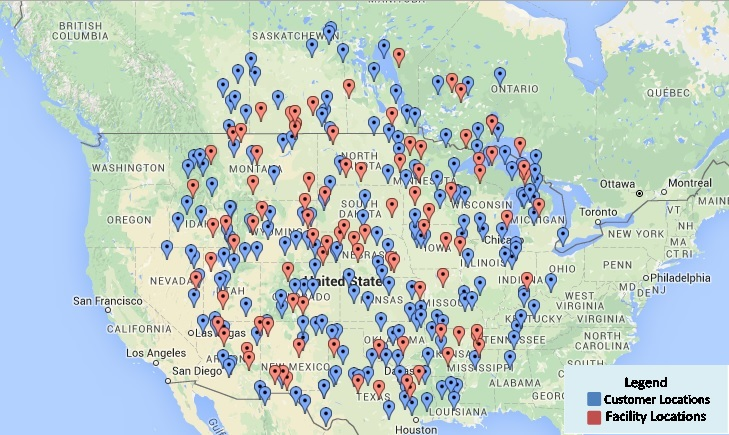
\includegraphics[width=\linewidth]{map.jpg}
  \caption{Facilities Open and Customers}
  \label{fig:optimalmap}
\end{figure}

\subsubsection{Results}
\begin{table}[H]
\centering
\caption{Capacitated (CFL) vs Uncapacitated (UFL)}
\label{comparison}
\resizebox{\linewidth}{!}{%
\begin{tabular}{|c|c|c|c|c|c|c|c|c|c|c|}
\hline
\multicolumn{3}{|c|}{\textbf{Data Set}} & \multirow{2}{*}{\textbf{\begin{tabular}[c]{@{}c@{}}Capacities \\ allowed\\ per facility\end{tabular}}} & \multicolumn{2}{c|}{\textbf{Facilities Open}} & \multicolumn{2}{c|}{\textbf{Total Cost}} & \multirow{2}{*}{\textbf{\% Difference}} & \multicolumn{2}{c|}{\textbf{Time}} \\ \cline{1-3} \cline{5-8} \cline{10-11} 
\textbf{\begin{tabular}[c]{@{}c@{}}No. of \\ facility \\ location\end{tabular}} & \textbf{\begin{tabular}[c]{@{}c@{}}No. of \\ customers\end{tabular}} & \textbf{\begin{tabular}[c]{@{}c@{}}No. of \\ parts\end{tabular}} &  & \textbf{UFL} & \textbf{CFL} & \textbf{UFL} & \textbf{CFL} &  & \textbf{UFL} & \textbf{CFL} \\ \hline
16 & 134 & 5 & 500-1000 & 7 & 9 & 294375.9714 & 344034.0172 & 16.87 & 0.578125 & 2.57863 \\ \hline
16 & 134 & 15 & 500-1000 & 9 & 14 & 436325.3109 & 697010.3145 & 59.75 & 1.343755 & 3.67525 \\ \hline
16 & 134 & 20 & 500-1000 & 9 & \begin{tabular}[c]{@{}c@{}}Integer \\ Infeasible\end{tabular} & 474348.4146 & \begin{tabular}[c]{@{}c@{}}Integer \\ Infeasible\end{tabular} & NA & 1.203125 & 4.09374 \\ \hline
16 & 134 & 20 & 1000-1500 & 9 & 11 & 474349.4146 & 549596.9598 & 15.86 & 1.203125 & 4.73437 \\ \hline
16 & 134 & 62 & 1000-1500 & 9 & 13 & 639485.6516 & 883105.4947 & 38.10 & 8.51562 & 11.42185 \\ \hline
16 & 134 & 62 & 1000-2500 & 9 & 11 & 639485.6516 & 690987.9552 & 8.05 & 8.51562 & 21.375025 \\ \hline
100 & 200 & 5 & 1000-1500 & 60 & 64 & 5223786.258 & 5321210.673 & 1.87 & 7.20312 & 33.296925 \\ \hline
100 & 200 & 5 & 500-1000 & 60 & 80 & 5223786.258 & 6135177.582 & 17.45 & 7.20312 & 16.5625 \\ \hline
\end{tabular}}
\end{table}
As expected, the results imply a cost increase when we change the problem to a CFLP, as well as the number of locations opened to satisfy the time based service level constraints also increase. This can be attributed to the fact that we have limited the capacity of each facility and thereby the number of parts it can hold. This in turn requires more than one facility to be opened in and around certain locations. We can observe that as the capacity of the facilities is increased, the cost reduces and less number of facilities are opened. Also, when it increases beyond the quantity required to satisfy the demand, the CFLP acts similar to that of UFLP as the capacity constraint acts like a redundant constraint in this case.\\
\begin{table}[H]
\centering
\caption{Variation of Cost \& Facilities with Total Capacity(16F*134C*5P)}
\label{capacity}
\begin{tabular}{|c|c|c|}
\hline
\textbf{Total Capacity Allowed} & \textbf{Facilities Open} & \textbf{Total Cost} \\ \hline
1000-2000 & 8 & 297990.0607 \\ \hline
500-2000 & 8 & 315302.5341 \\ \hline
500-1000 & 9 & 344034.0172 \\ \hline
400-800 & 11 & 380135.9238 \\ \hline
100-200 & \multicolumn{2}{c|}{Infeasible} \\ \hline
\end{tabular}
\end{table}
\begin{table}[H]
\centering
\caption{Variation of Cost \& Facilities with Part Capacity(16F*134C*5P)}
\label{parts}
\begin{tabular}{|c|c|c|}
\hline
\textbf{Part Capacity Allowed} & \textbf{Facilities Open} & \textbf{Total Cost} \\ \hline
500-600 & 8 & 303051.3576 \\ \hline
300-400 & 8 & 326466.3552 \\ \hline
200-300 & 11 & 350491.3767 \\ \hline
200-250 & 11 & 358795.0089 \\ \hline
150-200 & 16 & 576382.354 \\ \hline
100-200 & 16 & 18182189.66 \\ \hline
\end{tabular}
\end{table}
As we introduce part capacity, this limits the number of parts available at each location. We define the capacity of the facility as the sum of all the part capacities in the model. When we reduce the capacity per part per location, we are forced to open more facilities, leading to increased costs as shown in Table \ref{parts}. And when capacity reduces further, the problem is pushed towards infeasibility.\\
If we graph the variation of the number of facilities open against different part capacities allowed, we can observe that as we increase the capacity beyond 400 per part, for this specific demand, the model settles at 8 facilities shown in Figure \ref{fig:facparts}. Increasing capacity beyond this point has no effect on the number of facilities opened because of the distance parameters.\\
\begin{figure}[H]
\centering
  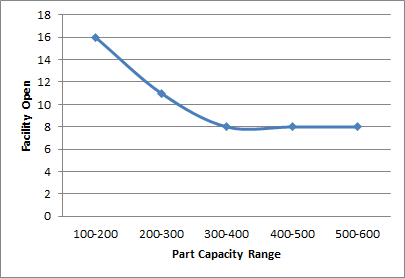
\includegraphics[scale=0.9]{Facilities.png}
  \caption{Variation of Facilities Open with Part Capacity}
  \label{fig:facparts}
\end{figure}
\begin{table}[H]
\centering
\caption{Variation of Cost with Number of Parts (Capacity:1000-1500)}
\begin{tabular}{|c|c|c|}
\hline
\textbf{Parts} & \textbf{UFL Cost (in \$mn)} & \textbf{CFL Cost (in \$mn)} \\ \hline
5 & 0.2943759714 & 0.304091998 \\ \hline
15 & 0.4363253109 & 0.4891344196 \\ \hline
20 & 0.4743494146 & 0.5495969598 \\ \hline
62 & 0.6394856516 & 0.8831054947 \\ \hline
\end{tabular}
\end{table}
\begin{figure}[H]
\centering
  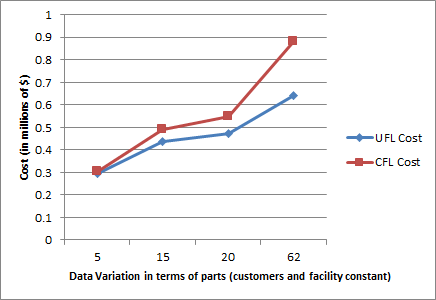
\includegraphics[scale=0.9]{Cost.png}
  \caption{Cost Comparison between UFL and CFL}
  \label{fig:Cost}
\end{figure}
Note that when the capacity is high, the CFLP is similar to UFL. The cost variations increases as the number of parts increase keeping the other parameters constant.
\begin{table}[H]
\centering
\caption{Variation of Cost \& Facilities with Demand (Constant Part capacity=100-200)}
\begin{tabular}{|c|c|c|}
\hline
\textbf{Demand} & \textbf{Facility Open} & \textbf{Cost} \\ \hline
0-20 & 72 & 16559433.98 \\ \hline
10 & 72 & 17701389.62 \\ \hline
10-20 & 72 & 25218825.89 \\ \hline
\end{tabular}
\end{table}
\begin{table}[H]
\centering
\caption{Variation of Cost \& Facilities with Demand (Constant Demand=20 units/part)}
\begin{tabular}{|c|c|c|}
\hline
\textbf{Capacity} & \textbf{Facility Open} & \textbf{Cost} \\ \hline
0-25 & \multicolumn{2}{c|}{Infeasible} \\ \hline
0-40 & \multicolumn{2}{c|}{Infeasible} \\ \hline
0-50 & 93 & 22780592.03 \\ \hline
20-25 & 81 & 17966683.94 \\ \hline
\end{tabular}
\end{table}
As part capacity reduces below a particular value, infeasibility sets in and when we increase the range of capacity i.e. if the part is unavailable at some locations, there will be adequate quantity available at some other location to satisfy the demand but at the expense of a higher cost.\\
Although mathematical models of those problems are not very different from the UFL models, the solving methods for CFLP are more difficult. Due to the progress in technology of the solvers like CPLEX, it is now possible to solve CFLP instances with up to 100 facilities, 5 parts and 300 clients on personal computers. Above this problem size exact solution becomes prohibitive and we use the LP-relaxation along with rounding techniques to find a near optimal solution. \\
\subsubsection{LP Relaxation Solution}
The smaller instances of the problem which are difficult to be solved as IP’s using CPLEX, are solved to get an acceptable bound by solving the LP relaxation of the IP and then rounding the non-integer variables to the nearest integer. This technique can be effectively used for problems of larger sizes when compared to IP but not huge problems. The technique is briefly described below using an instance for 100 locations, 200 customers and 200 parts.\\

Problem Size: F=100 C=200 P=200\\
Capacity=uniform(0,50)\\
Demand=uniform(0,20)\\

\begin{table}[H]
\centering
\caption{Comparison of IP with LP}
\resizebox{\linewidth}{!}{%
\begin{tabular}{|c|c|c|c|c|}
\hline
 & \textbf{IP optimal value} & \textbf{LP relaxed solution} & \textbf{Variables fixed/rounded} & \textbf{\% Error} \\ \hline
\multirow{2}{*}{\textbf{Cost}} & \multirow{2}{*}{\begin{tabular}[c]{@{}c@{}}Optimal value: 22780592.03\\ Facilities Open: 93\end{tabular}} & \begin{tabular}[c]{@{}c@{}}LP1: 22772636.71\\ Facilities Open: 89\end{tabular} & \begin{tabular}[c]{@{}c@{}}FacilityOpen{[}32{]}=1 (Open)\\ FacilityOpen{[}54{]}=1 (Open)\\ FacilityOpen{[}73{]}=1 (Open)\end{tabular} & 0.04 \\ \cline{3-5} 
 &  & \begin{tabular}[c]{@{}c@{}}LP2: 22773562.02\\ Facilities Open: 92\end{tabular} & - & 0.03 \\ \hline
\end{tabular}}
\end{table}
As the problem size increases, it becomes more difficult to solve the LP relaxation to find the optimal solution. Therefore, we apply a simple and effective heuristic based on a Lagrangian relaxation along with variable fixing. This is used to derive a tighter bound on the optimal value of the problem in this project.

\subsubsection{Lagrangian relaxation of CFLP}
Consider the Lagrangian relaxation of the demand constraints by using lagrangian multipliers $\lambda_{ik}$. The Lagrangian relaxation of the constraint reduces the relaxed problem to a knapsack problem which gives a better bound than the LP relaxation. Updated model: \\
\begin{equation}
\label{obj}
z(\lambda)= Min \sum_{i\in I}f_{i}Y_{i} + \sum_{i\in I}\sum_{j\in J}\sum_{k\in K}c_{ijk}d_{jk}X_{ijk} + \sum_{i\in I, k\in K}\lambda_{ik}(1-\sum_{i\in I}X_{ijk})
\end{equation}
\hspace{2cm} subject to
\begin{equation}
\label{supply}
X_{ijk} \leq Y_{i},  \forall i,j,k  
\end{equation}
\begin{equation}
\label{compound}
\sum_{i\in I}\sum_{j\in J}\frac{\delta_{ijw}d_{jk}X_{ijk}}{d_k} \geq \alpha_{kw},  \forall k,w  
\end{equation}
\begin{equation}
\label{Fraction}
0 \leq X_{ijk} \leq 1,  \forall i,j,k  
\end{equation}
\begin{equation}
\label{Indicator}
Y_{i} \in \{0,1\}, \forall i 
\end{equation}
\begin{equation}
\label{FacCapacity}
\sum_{j\in J}\sum_{k\in K} d_{jk}X_{ijk} \leq Y_{i}h_{i},    \forall i
\end{equation}
\begin{equation}
\label{PartCapacity}
\sum_{j\in J} d_{jk}X_{ijk} \leq Y_{i}g_{ik},    \forall i,k
\end{equation}

The Lagrangian function is maximized by subgradient optimization. The subgradient algorithm is used in conjunction with step-size rule to achieve convergence to a fairly good lower bound in less than 250 iterations.\\
We use the subgradient method to determine the set $\lambda^{*}$ which maximizes the Lagrangian function. The subgradient method generates a sequence of Lagrangian multipliers for the relaxed constraint $A^{1}x=b^{1}$ which is given by:
$$\lambda^{k+1} = \lambda^{k}+ \theta_{k}(b^{1}-A^{1}x^{k})_{i}$$
where 
$$\theta_{k}=\alpha_{k}(w_{LB}-z(\lambda^{k}))/\sum_{i}(b^{1}-A^{1}x^{k})_{i}^{2}$$

An instance solved using Lagrangian relaxation for a data size of:\\
F=100 C=200 P=200\\
Capacity=uniform(0,50)\\
Demand=uniform(0,20)\\

\begin{table}[H]
\centering
\caption{Comparison of IP with LR}
\label{my-label}
\begin{tabular}{|c|c|c|c|}
\hline
\textbf{} & \textbf{IP solution} & \textbf{LR solution} & \multicolumn{1}{l|}{\textbf{\% Error}} \\ \hline
\textbf{Cost} & 22780592.03 & 22735038.85 & 1.99 \\ \hline
\textbf{Facilities Open} & 93 & 93 & - \\ \hline
\end{tabular}
\end{table}
The Lagrangian relaxation solves a problem of size 100*200*200 within an error of 2\% (approx.) without sufficient improvement in time, suggesting that as the problem size increases, solving the relaxation still requires solving of an IP which still has the time-based constraints. Note that if we relax more constraints to attain easy solvability, we may reduce the time required to solve the model but results in worse bounds.
\section{Model II: Multi-Echelon Distribution Network}
In this section we have designed a two-echelon distribution network with a hub at the first echelon and potential local warehouse locations at the second echelon \cite{CH}.
\subsection{Basic Model}
Parameters:
\begin{itemize}
\item 
Candidate Location for Hubs: Set I indexed by i
\item 
Customers or Demand Points: Set J indexed by j
\item 
Parts: Set K indexed by k
\item
Warehouses: Set L indexed by l
\item
Service window levels: Set W indexed by w 
\item
Transportation cost between hub i and warehouse l: $p_{il}$
\item
Fixed cost of opening a hub: $f_i$
\item
Fixed cost of opening a warehouse: $g_l$
\item 
Transportation cost between warehouse l and customer j for part k: $c_{lj}$
\item 
Demand for part k at location/customer j: $d_{jk}$
\item
Total demand rate for part k: $d_{k} = \sum_{j\in J}d_{jk}$
\item
Service level for part k: $\alpha_{jkw}$
\item
Identifier $\delta_{ijw} = 1$, if facility i can ship a part requested at demand point j within the specified service time window, 0 otherwise  
\end{itemize}

Decision Variables:
\begin{itemize}
\item
$Y_i = 1$ if hub i is open, 0 otherwise
\item
$Z_l = 1$ if warehouse l is open, 0 otherwise
\item
Demand for part k at hub i from warehouse l: $V_{lik}$
\item
Fraction of demand met for part k from warehouse l for customer j: $X_{ljk}$
\end{itemize}
Please note that $\alpha$ is a parameter and can take any value in $(0,1]$ in this model. This $\alpha$ value once set is the same for all parts. Overall model is as follows:

\begin{equation}
Min \sum_{i\in I}f_{i}Y_{i} + \sum_{l\in L}g_{l}Z_{l} + \sum_{i\in I,l \in L, k \in K}p_{il}V_{lik} + \sum_{l\in L, j \in J, k \in K}c_{lj}X_{ljk}d_{jk}
\end{equation}
\hspace{2cm} subject to
\begin{equation}
\sum_{l\in L}X_{ljk} = 1,  \forall j,k  
\end{equation}
\begin{equation}
X_{ljk} \leq Z_{l},  \forall j,k,l
\end{equation}
\begin{equation}
V_{lik} \leq MY_{i},  \forall i,k,l
\end{equation}
\begin{equation}
\sum_{i\in I} V_{lik} \geq \sum_{j \in J} X_{ljk}d_{jk}  \forall k,l
\end{equation}
\begin{equation}
\sum_{l\in L} X_{ljk}\frac{d_{jk}}{d_{k}}\delta_{ijw} \geq \alpha_{jkw}  \forall j,k,w
\end{equation}
\begin{equation}
0 \leq X_{ljk} \leq 1,  \forall j,k,l 
\end{equation}
\begin{equation}
\label{Indicator}
Y_{i} \in \{0,1\}, \forall i, 
Z_{l} \in \{0,1\}, \forall l
\end{equation}
\subsection{Results}
The problem was solved for the following instance:\\
Hubs=50, Warehouses=150, Customers=200, Parts=10\\
\textbf{Optimal cost: 5170764.031\\
Hubs Open: 22\\
Warehouses Open:62}
\begin{figure}[H]
\centering
  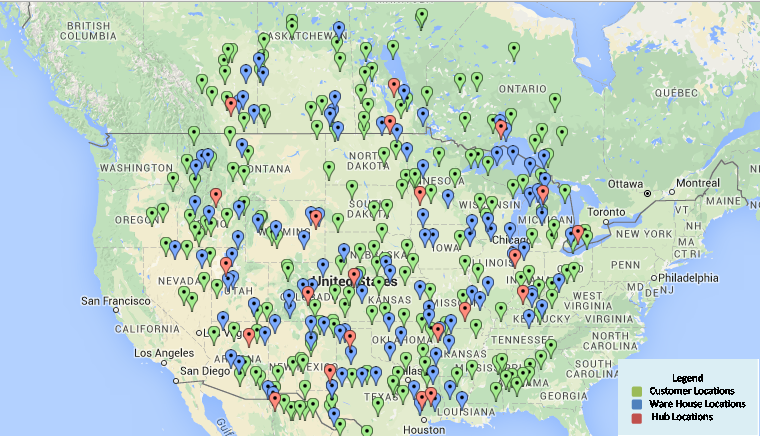
\includegraphics[scale=0.63]{hubmap.png}
  \caption{Customers, open hubs and open warehouses}
  \label{fig:hubwh}
\end{figure}
The two-echelon model considers service levels between the warehouses and customers and we assume no direct supply from hubs to customer locations. The instance solved, suggests opening 62 warehouses and 22 hubs to supply to these, incurring a total cost of \$5,170,764 for a specified service level alpha as shown in Figure \ref{fig:hubwh}. The model took 6 hours to solve the problem of given size, suggesting that model complexity increases as more constraints are included in the model.
\section{Conclusion}
In this project, we considered a logistic network design problem with time-based service requirements as a UFLP, CFLP and a two echelon system. We solved different instances of the LND problem as UFLP and CFLP and outlined the basic difference in these two models in terms of the increase in the cost as well as the computational difficulty. We conducted extensive computational tests using instances based on the data generated to quantify the differences in UFLP and CFLP.\\

It is quite evident from the results that as we add capacity to the UFLP problem, the cost increased as well as the number of facilities to be opened to meet the service level requirements. Also, the UFLP for large networks is solved easily with CPLEX in matter of minutes but as we move on to the CFLP, a medium sized problem itself takes hours to solve in CPLEX using a personal laptop. This may be improved if we use systems with high processing power but the availability of heuristic methods makes it appealing to solve the relaxed version of the problem, which in our case provided a bound within 2.5\% of the optimal value.\\ 

Our lagrangian heuristic provided a value within 2.5\% whereas the lagrangian relaxation for CFLP is expected to give an optimal value within 1.25\% of the actual optimal value \cite{CFL}. The variation in our bound could be because of the extra service level constraints, which changes the problem as compared to a normal CFLP. \\
\section{Future Scope}
Converting the problem to a multi-echelon system is an interesting part we covered in the model. But we have designed a two echelon model in this project but it could be improved further. This can be used to effectively models real life scenarios in which actual warehouses operate. This model could be further investigated by adding multiple levels to this model. Interesting scenarios like wholesale procurement and transportation intricacies like fleet availability, transportation using full truck capacity, less than full truck capacity etc.can be effectively modelled into this kind of system and solved to get easily implementable and realistic solutions.The main drawback with this model is its high computational requirements and the new model takes much time to solve compared to the models described in this project. But heuristic methods could always be used to find feasible and near optimal solutions in less time.
\newpage
\addcontentsline{toc}{section}{References}
\begin{thebibliography}{99}
\bibitem{EK} Mehmet Ferhat Candas and Erhan Kutanoglu, {\em Benefits of Considering Inventory in Service Parts Logistics Network Design Problems with Time-based Service Constraints}. IIE Trans, v.39, p.159, 2007.
\bibitem{SD} S. David Wu and Hakan Golbasi, {\em Multi-Item, Multi-Facility Supply Chain Planning: Models, Complexities, and Algorithms}. Computational Optimization and Applications, v.28, p.325-356, 2004.
\bibitem{CD} Mehmet Ferhat Candas, {\em Considering inventory in service parts logistics network design problems with time-based service constraints}. PhD dissertation. The University of Texas at Austin, 2007.
\bibitem{AV} Pasquale Avella, Maurizio Boccia, Antonio Sforza and Igor Vasil’ev, {\em An effective heuristic for large-scale capacitated facility location problems}. Springer Science Journal of Heuristics, v.15, p.597–615, 2009.
\bibitem{CH} Michelle L.F. Cheong, Rohit Bhatnagar and Stephen C. Graves, {\em Logistics network design with supplier consolidation hubs and multiple shipment options}. Journal of Industrial and Management Optimization, v.3, p.51, 2007.
\bibitem{CFL} Pasquale Avella, Maurizio Boccia, Antonio Sforza and Igor Vasil’ev, {\em An effective heuristic for large-scale capacitated facility location problems}. Journal of Heuristics, v.15, p.597-615, 2009.
\bibitem{random} "Random Point Generator With Maps". Website, 2016. \url{http://geomidpoint.com/random/}
\end{thebibliography}
%%%%%%%%%%%%%%%%%%%%
\newpage
\appendix
\addcontentsline{toc}{section}{APPENDIX}
\section{AMPL Code}
\label{code}
\subsection{Model in AMPL}
\textbf{\underline {Mod file:}}\\
\begin{verbatim}
param I >= 0; # No. of Customers
param J >= 0; # No. of Facilities
param K >= 0; # No. of Parts
param SL >= 0; # Number of Service Level
param cost{i in 1..I, j in 1..I, k in 1..K} >= 0; #Cost of transportation
param Demand{i in 1..I, k in 1..K} >= 0; # Demand of part k at a Customer i
param ProdDemand{k in 1..K} = sum{i in 1..I} Demand[i,k];
param FacilityCost{j in 1..J} := 10000; # Facility Fixed Cost
param alpha{k in 1..K, s in 1..SL} :=0.5; # Fixed Service Level
param delta{i in 1..I, j in 1..J, s in 1..SL} >= 0; 
#param ReachFactor {f in 1..F, c in 1..C} >= 0; # Reach Factor 
                                                        

var FacilityOpen{j in 1..J} binary; # Facility Open or not
var FracDemand{i in 1..I, j in 1..J, k in 1..K} >= 0;

minimize TotalCost:
sum{j in 1..J} FacilityCost[j]*FacilityOpen[j] + 
sum{i in 1..I, j in 1..J, k in 1..K} cost[j,i,k]*Demand[i,k]*FracDemand[j,i,k];

subject to Demand_Constraint {i in 1..I, k in 1..K}:
sum{j in 1..J} FracDemand[j,i,k] = 1;

subject to Supply_if_FacilityOpen {i in 1..I, j in 1..J, k in 1..K}:
FracDemand[j,i,k] <= FacilityOpen[j];   #Disaggregated

#subject to SupplyifFacilityOpen {f in 1..F, p in 1..P}: #Alternate Model
#sum{c in 1..C} FracDemand[f,c,p] <=c*FacilityOpen[f];  #Aggregated 

subject to Service_Delta_Contraint {k in 1..K, s in 1..SL}:
sum{i in 1..I, j in 1..J} FracDemand[j,i,k]*
                (Demand[i,k]/ProdDemand[k])*delta[j,i,k] >= alpha[k,s];

#subject to FracDemandConstraint {i in 1..I, j in 1..J, k in 1..K}:
#FracDemand[j,i,k] <= ReachFactor[f,c];     # Reach Factor 
\end{verbatim}
\textbf{\underline{Dat file:}}
\begin{verbatim}
param I := 134;  # No. of Customers
param J:= 16;   # No. of Facilities
param K := 15;  # No. of Parts
#param K := 5;
#param K := 20;
#param K := 62;
param SL := 3; # Number of Service Level
param Demand:=<Demand matrix>
param delta:=<delta matrix>
param cost:= <cost matrix>
#param ReachFactor:= <Reach matrix>   # Reach Factor

\end{verbatim}
\subsection{Tiered Service levels and Restricted Facility Open}
\textbf{\underline{Mod file:}}
\begin{verbatim}
param I >= 0; # No. of Customers
param J >= 0; # No. of Facilities
param K >= 0; # No. of Parts
param SL >= 0; # Number of Service Level
param cost{i in 1..I, j in 1..I, k in 1..K} >= 0; #Cost of transportation
param Demand{i in 1..I, k in 1..K} >= 0; # Demand of part k at a Customer i
param ProdDemand{k in 1..K} = sum{i in 1..I} Demand[i,k];
param FacilityCost{j in 1..J} := 10000; # Facility Fixed Cost
param alpha{k in 1..K, s in 1..SL} >= 0; # Varying Service Level
param delta{i in 1..I, j in 1..J, s in 1..SL} >= 0; 
#param TotalFacilityOpen >= 0; #Restricted Facility Opening

var FacilityOpen{j in 1..J} binary; # Facility Open or not
var FracDemand{i in 1..I, j in 1..J, k in 1..K} >= 0;

minimize TotalCost:
sum{j in 1..J} FacilityCost[j]*FacilityOpen[j] + 
sum{i in 1..I, j in 1..J, k in 1..K} cost[j,i,k]*Demand[i,k]*FracDemand[j,i,k];

subject to Demand_Constraint {i in 1..I, k in 1..K}:
sum{j in 1..J} FracDemand[j,i,k] = 1;

subject to Supply_if_FacilityOpen {i in 1..I, j in 1..J, k in 1..K}:
FracDemand[j,i,k] <= FacilityOpen[j];

subject to Service_Delta_Contraint {k in 1..K, s in 1..SL}:
sum{i in 1..I, j in 1..J} FracDemand[j,i,k]*
                    (Demand[i,k]/ProdDemand[k])*delta[j,i,k] >= alpha[k,s];
                    
#subject to NumberofFacilities:     # Restricted facility opening
#sum{f in 1..F} FacilityOpen[f] <= TotalFacilityOpen;

subject to FracDemandConstraint {i in 1..I, j in 1..J, k in 1..K}:
FracDemand[j,i,k] <= 1;
\end{verbatim}
\textbf{\underline{Dat file:}}
\begin{verbatim}
param I := 134;  # No. of Customers
param J:= 16;   # No. of Facilities
param K := 15;  # No. of Parts
#param K := 5;
#param K := 20;
#param K := 62;
param SL := 3; # Number of Service Level
param Demand:=<Demand matrix>
param delta:=<delta matrix>
param cost:= <cost matrix>
param alpha:= <alpha matrix>
\end{verbatim}
\subsection{Capacitated Facility Location Problem}
\textbf{\underline{Mod file:}}
\begin{verbatim}
param C >= 0; # No. of Customers
param F >= 0; # No. of Facilities
param P >= 0; # No. of Parts
param W >= 0; # No of service window
param CPD := 20; #cost per unit distance
param distance{f in 1..F, c in 1..C} >= 0; #Cost
param Demand{c in 1..C, p in 1..P} := 
                floor(Uniform(10,500)); #Part Demand at a Customer
param ProdDemand{p in 1..P} = sum{c in 1..C} Demand[c,p];
param FacilityCost{f in 1..F} :=10000; # Facility Fixed Cost
param alpha{p in 1..P,w in 1..W}>=0; # Service Level
param delta{f in 1..F, c in 1..C, w in 1..W} >=0; #
param part_capacity{f in 1..F,p in 1..P}:= floor(Uniform(200,250));
#param part_capacity{f in 1..F,p in 1..P}:= floor(Uniform(0,250));
param fac_capacity{f in 1..F}:= sum {p in 1..P} part_capacity[f,p];

var FacilityOpen{f in 1..F} binary; # Facility Open or not
var FracDemand{f in 1..F, c in 1..C, p in 1..P} >= 0;

minimize TotalCost:
sum{f in 1..F} FacilityCost[f]*FacilityOpen[f] + 
sum{f in 1..F, c in 1..C, p in 1..P} CPD*distance[f,c]*
                                    Demand[c,p]*FracDemand[f,c,p];

subject to DemandConstraint {c in 1..C, p in 1..P}:
sum{f in 1..F} FracDemand[f,c,p] = 1;

subject to SupplyifFacilityOpen {f in 1..F, c in 1..C, p in 1..P}: 
FracDemand[f,c,p] <= FacilityOpen[f];   #Disaggregated

#subject to SupplyifFacilityOpen {c in 1..C, p in 1..P}: # Aggregated
#sum{f in 1..F}FracDemand[f,c,p] <= C*FacilityOpen[f];

subject to ServiceLevelSatisfiedConstraint {p in 1..P, w in 1..W}:
sum{f in 1..F, c in 1..C} FracDemand[f,c,p]*
                (Demand[c,p]/ProdDemand[p])*delta[f,c,w] >= alpha[p,w];

subject to FracDemandConstraint {f in 1..F, c in 1..C, p in 1..P}:
FracDemand[f,c,p] <= 1;

subject to sumpartcapacity {f in 1..F}: 
sum {p in 1..P}part_capacity[f,p] <= 
    fac_capacity[f];  #sum part capacity less than facility capacity

subject to capacityconstraint {f in 1..F}: #simple capacity constraint
sum{c in 1..C, p in 1..P} Demand[c,p]*FracDemand[f,c,p]                                                          <=FacilityOpen[f]*fac_capacity[f];

subject to partcapacityconstraint {f in 1..F, p in 1..P}: 
sum{c in 1..C} Demand[c,p]*FracDemand[f,c,p] <= FacilityOpen[f]*
                    part_capacity[f,p]; #partwise capacity constraint
\end{verbatim}
\textbf{\underline{Dat file:}}
\begin{verbatim}
param C := 300; # No. of Customers
param F := 50; # No. of Facilities
param P := 200; # No. of Products
param W := 3; # No of service window
param alpha:= <alpha matrix>
param distance:= <distance matrix>
param delta:= <delta matrix>
\end{verbatim}
\subsubsection{Lagrangian Relaxation of CFLP}
\textbf{\underline{Mod file:}}
\begin{verbatim}
param C >= 0; # No. of Customers
param F >= 0; # No. of Facilities
param P >= 0; # No. of Products
param W >= 0; # No of service window
#param CPD := 20; #cost per unit distance
param distance{f in 1..F, c in 1..C, p in 1..P} >= 0; #Cost
param Demand{c in 1..C, p in 1..P} >= 0;
#param Demand{c in 1..C, p in 1..P} := 
floor(Uniform(0,20)); # Product Demand at a Customer
param ProdDemand{p in 1..P} = sum{c in 1..C} Demand[c,p];
param FacilityCost{f in 1..F} := 10000; # Facility Fixed Cost
param alpha{p in 1..P,w in 1..W} >= 0; # Service Level
param delta{f in 1..F, c in 1..C, w in 1..W} >= 0; #Using Only Service Window 1
param part_capacity{f in 1..F,p in 1..P}:= floor(Uniform(100,200));
#param part_capacity{f in 1..F,p in 1..P}:= floor(Uniform(0,250));
param fac_capacity{f in 1..F}:= sum {p in 1..P} part_capacity[f,p];
param u{c in 1..C, p in 1..P} >= 0; #Lagrangian multipliers

var FacilityOpen{f in 1..F} binary; # Facility Open or not
var FracDemand{f in 1..F, c in 1..C, p in 1..P} >= 0<=1;

minimize Lagrangian:
sum{f in 1..F} FacilityCost[f]*FacilityOpen[f] + 
sum{f in 1..F, c in 1..C, p in 1..P} distance[f,c,p]*
Demand[c,p]*FracDemand[f,c,p]+
sum {c in 1..C, p in 1..P} u[c,p]*
(1-sum {f in 1..F} FracDemand[f,c,p]);

minimize TotalCost:
sum{f in 1..F} FacilityCost[f]*FacilityOpen[f] + 
sum{f in 1..F, c in 1..C, p in 1..P} distance[f,c,p]*
Demand[c,p]*FracDemand[f,c,p];

subject to DemandConstraint {c in 1..C, p in 1..P}:
sum{f in 1..F} FracDemand[f,c,p] = 1;

subject to SupplyifFacilityOpen {f in 1..F, c in 1..C, p in 1..P}: 
FracDemand[f,c,p] <= FacilityOpen[f]; #Disaggregated

subject to ServiceLevelSatisfiedConstraint {p in 1..P, w in 1..W}:
sum{f in 1..F, c in 1..C} FracDemand[f,c,p]*
            (Demand[c,p]/ProdDemand[p])*delta[f,c,w] >= alpha[p,w];

subject to capacityconstraint {f in 1..F}: #simple capacity constraint
sum{c in 1..C, p in 1..P}Demand[c,p]*
                FracDemand[f,c,p]<=FacilityOpen[f]*fac_capacity[f];

#subject to partcapacityconstraint {f in 1..F, p in 1..P}: 
#sum{c in 1..C} Demand[c,p]*FracDemand[f,c,p] <= FacilityOpen[f]*
part_capacity[f,p];   #partwise capacity constraint
\end{verbatim}
\textbf{\underline{Dat file:}}
\begin{verbatim}
param C := 300; # No. of Customers
param F := 50; # No. of Facilities
param P := 200; # No. of Products
param W := 3; # No of service window
param alpha:= <alpha matrix>
param distance:= <distance matrix>
param delta:= <delta matrix>
\end{verbatim}
\subsection{Model II: Multi-Echelon Distribution Network}
\textbf{\underline{Mod file:}}
\begin{verbatim}
param C >= 0; #
param C >= 0; # No. of Customers
param H >= 0; # No. of Facilities
param P >= 0; # No. of Products
param W >= 0; # Number of Service Level
param WH >= 0; # No of ware houses
param cost_HtoWH {h in 1..H, wh in 1..WH} >= 0; # Cost ub to warehouse
param cost_WHtoC {wh in 1..WH, c in 1..C} >=0; # cost Warehouse to customer
param Demand {c in 1..C, p in 1..P} := 
            floor(Uniform(10,20)); # Product Demand at a Customer
param ProdDemand{p in 1..P} = sum{c in 1..C} Demand[c,p];
param HubCost{h in 1..H} := 10000; # Facility Fixed Cost
param WHCost {wh in 1..WH} := 5000; # Warehouse opening cost
param alpha{p in 1..P, w in 1..W} =0.5; # Service Level (to be generated)
param delta{wh in 1..WH, c in 1..C, w in 1..W} 
                            >= 0; # Using Only Service Window 1
param M := 1000000; #Big M

var HubOpen {h in 1..H} binary; # Hub Open or not
var WarehouseOpen {wh in 1..WH} binary; # Warehouse open or not
var HubDemand {h in 1..H, wh in 1..WH, p in 1..P} >= 0;
var WHFracDemand {wh in 1..WH, c in 1..C, p in 1..P} >=0 <=1;
#var WHDemand {wh in 1..WH, p in 1..P} >=0;

minimize TotalCost:
sum{h in 1..H} HubCost[h]*HubOpen[h] + 
sum {wh in 1..WH} WHCost[wh]*WarehouseOpen[wh] +
sum {h in 1..H, wh in 1..WH, p in 1..P} cost_HtoWH[h,wh]* 
HubDemand[h,wh,p] + sum{wh in 1..WH, c in 1..C, p in 1..P} 
cost_WHtoC[wh,c]* WHFracDemand[wh,c,p] * Demand[c,p];

subject to Cust_DemandSatisfied {c in 1..C, p in 1..P}:
	sum {wh in 1..WH} WHFracDemand[wh,c,p] = 1;

subject to DemandConstraint {wh in 1..WH, p in 1..P}:
	sum {h in 1..H} HubDemand [h,wh,p]>= sum{c in 1..C} 
	                        WHFracDemand[wh,c,p] * Demand[c,p];

subject to SupplyifHubOpen {h in 1..H, wh in 1..WH, p in 1..P}: 
	HubDemand[h,wh,p] <= HubOpen[h] * M;  #Disaggregated
	
subject to SupplyifWHOpen {wh in 1..WH, c in 1..C, p in 1..P}:
	WHFracDemand[wh,c,p] <= WarehouseOpen[wh];

subject to ServiceLevelConstraint {p in 1..P, w in 1..W}:
	sum{wh in 1..WH, c in 1..C} WHFracDemand[wh,c,p]*(Demand[c,p]/ProdDemand[p])*
	                            delta[wh,c,w] >= alpha[p,w];

#subject to NumberofFacilities: # Point 6th Constriant
#sum{f in 1..F} FacilityOpen[f] <= TotalFacilityOpen;
\end{verbatim}
\textbf{\underline{Dat file:}}
\begin{verbatim}
param C := 200; # No. of Customers
param H := 50; # No. of Facilities
param P := 5; # No. of Products
param W := 3; # Number of Service Level
param WH := 150; # No of ware houses
param cost_HtoWH :=<distance matrix>
param cost_WHtoC :=<distance matrix>
param delta:= <delta matrix>
\end{verbatim}
\section{Python Codes}
\subsection{Distance Calculation}
\begin{verbatim}
import openpyxl
import numpy as np
import math
from haversine import haversine
wb = openpyxl.load_workbook('//home//archit//Distance.xlsx')
count=2
for i in range(1,1001):
    for j in range(1,1001):
        dist['A'+str(count)].value=i
        dist['B'+str(count)].value=j
        facility=(fac['B'+str(i+1)].value,fac['C'+str(i+1)].value)
        customer=(cust['B'+str(j+1)].value,cust['C'+str(j+1)].value)
        dist['C'+str(count)].value = haversine(facility,customer,miles=True)
        count+=1
wb.save('//home//archit//Distance.xlsx')
\end{verbatim}
\subsection{Delta Calculation}
\begin{verbatim}
import openpyxl
import numpy as np
import math
from haversine import haversine
wb = openpyxl.load_workbook('//home//archit//Delta.xlsx')
delta=wb.get_sheet_by_name('Delta')
fac=wb.get_sheet_by_name('Facilities')
cust=wb.get_sheet_by_name('Customers')
count=2
for i in range(1,101):
    for j in range(1,201):
        for k in range(1,4):
            facility=(fac['B'+str(i+1)].value, fac['C'+str(i+1)].value)
            customer=(cust['B'+str(j+1)].value, cust['C'+str(j+1)].value)
            delta['A'+str(count)].value=k
            delta['B'+str(count)].value=i
            delta['C'+str(count)].value=j
            if (k==1):
                if(haversine(facility, customer, miles=True)<280):
                    delta['D'+str(count)].value=1
                    count+=1
                    for l in range(2,4):
                        delta['A'+str(count)].value=l
                        delta['B'+str(count)].value=i
                        delta['C'+str(count)].value=j
                        delta['D'+str(count)].value=1
                        count+=1
                    break
                else: 
                    delta['D'+str(count)].value=0
            elif(k==2):
                if(haversine(facility, customer, miles=True)<840):
                    delta['D'+str(count)].value=1
                else:
                    delta['D'+str(count)].value=0
            elif(k==3):
                if(haversine(facility, customer, miles=True)<5040):
                    delta['D'+str(count)].value=1
                else:
                    delta['D'+str(count)].value=0
            count+=1
wb.save('//home//archit//Delta.xlsx')
\end{verbatim}
\end{document}